% Generated by make_fig_pdg.py from programs/*.py and the study's code. Do not edit by hand.
\documentclass[border=2pt]{standalone}
\usepackage[T1]{fontenc}\usepackage{newtxtext,newtxmath}\usepackage[varqu,scaled=0.95]{zi4}
\usepackage{amsmath,xcolor,listings,tikz}\usetikzlibrary{arrows.meta,calc,patterns}
\definecolor{cblue}{HTML}{0072B2}\definecolor{cver}{HTML}{D55E00}\definecolor{cgreen}{HTML}{009E73}
\definecolor{cpurple}{HTML}{7E57C2}
\definecolor{lvA}{HTML}{24527F}\definecolor{lvB}{HTML}{86B6DD}\definecolor{lvC}{HTML}{FFE27A}
\lstdefinestyle{qiskit}{language=Python,basicstyle=\ttfamily\fontsize{7.6}{9.4}\selectfont,numbers=left,
  numberstyle=\fontsize{6}{7}\selectfont\color{black!55},numbersep=3pt,keywordstyle=\color{cblue}\bfseries,
  commentstyle=\color{black!55}\itshape,showstringspaces=false,frame=single,rulecolor=\color{black!25},
  xleftmargin=13pt,framexleftmargin=11pt,framerule=0.4pt,columns=flexible,keepspaces=true,aboveskip=0pt,belowskip=0pt}
\tikzset{
  op/.style={rectangle, rounded corners=2pt, draw=black!60, line width=0.45pt, fill=white, align=center,
             inner xsep=2pt, inner ysep=1.3pt, font=\ttfamily\fontsize{6}{6.6}\selectfont},
  insl/.style={op, fill=cblue!22},
  missdep/.style={op, draw=cver, line width=0.9pt, dash pattern=on 1.6pt off 1pt},
  missdepsl/.style={missdep, fill=cblue!22},
  entx/.style={op, fill=cpurple!30, draw=cpurple, line width=0.8pt},
  lvdu/.style={op, fill=lvA, draw=black!80, text=white},
  lvcp/.style={op, fill=lvB, draw=black!70},
  lvqd/.style={op, fill=lvC, draw=black!70},
  entxh/.style={op, fill=cver!22, draw=cver, line width=0.9pt},
  clq/.style={cl, fill=black!14, draw=black!60},
  cpdgE/.style={-{Stealth[length=1.3mm]}, draw=black, line width=0.8pt, line cap=round, dash pattern=on 0pt off 1.7pt},
  crit/.style={double=white, double distance=0.7pt, line width=0.5pt},
  dataE/.style={-{Stealth[length=1.2mm]}, draw=black!50, line width=0.45pt},
  quantumE/.style={-{Stealth[length=1.4mm]}, draw=cblue, line width=1.1pt},
  controlE/.style={-{Stealth[length=1.3mm]}, draw=cgreen, line width=0.85pt, dash pattern=on 2.2pt off 1.1pt},
  missingE/.style={-{Stealth[length=1.3mm]}, draw=cver, line width=0.85pt, dash pattern=on 1.8pt off 1.2pt},
  ttl/.style={font=\footnotesize\bfseries, anchor=south},
  cl/.style={op, draw=black!45, fill=black!4, font=\ttfamily\fontsize{7.6}{8.4}\selectfont},
  clsl/.style={cl, fill=cblue!22, draw=black!60},
  loopbox/.style={draw=black!40, rounded corners=3pt, line width=0.5pt, dash pattern=on 2.5pt off 1.2pt},
  boxlbl/.style={font=\ttfamily\fontsize{7.2}{7.8}\selectfont, text=black!65, inner sep=1pt},
  note/.style={font=\scriptsize, anchor=north, align=center},
}
\begin{document}
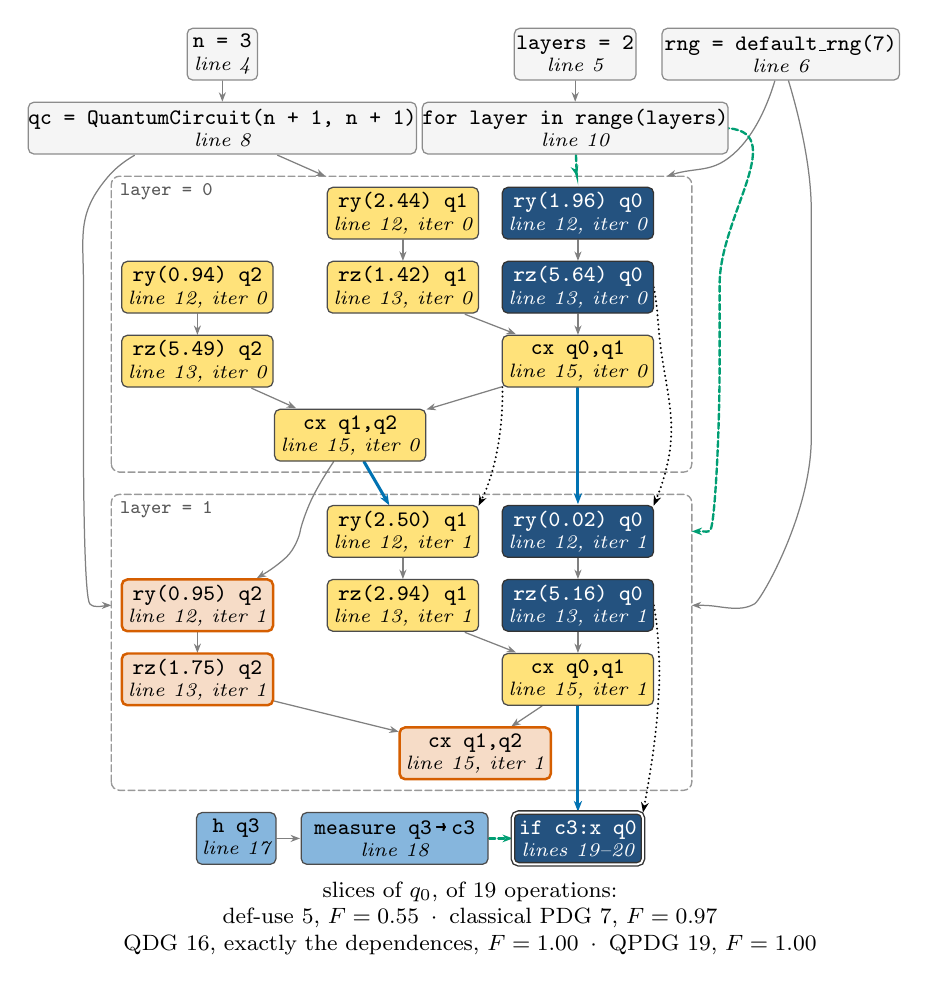
\begin{tikzpicture}[line cap=round]
  \draw[loopbox] (0.898,-5.637) rectangle (8.271,-1.879);
  \node[boxlbl, anchor=north west] at (0.969,-1.936) {layer = 0};
  \draw[loopbox] (0.898,-9.678) rectangle (8.271,-5.920);
  \node[boxlbl, anchor=north west] at (0.969,-5.976) {layer = 1};
  \draw[cpdgE] (7.789,-3.289) .. controls (7.789,-3.289) and (7.827,-3.500) .. (7.838,-3.670) .. controls (7.902,-4.655) and (8.187,-5.005) .. (7.846,-5.914) -- (7.786,-6.064);
  \draw[cpdgE] (5.865,-4.557) .. controls (5.865,-4.557) and (5.900,-5.291) .. (5.637,-5.910) -- (5.563,-6.064);
  \draw[cpdgE] (7.789,-7.329) .. controls (7.789,-7.329) and (7.827,-7.540) .. (7.838,-7.711) .. controls (7.865,-8.127) and (7.868,-8.234) .. (7.838,-8.650) .. controls (7.809,-9.063) and (7.728,-9.543) .. (7.683,-9.791) -- (7.651,-9.960);
  \draw[dataE] (6.825,-2.688) .. controls (6.825,-2.726) and (6.825,-2.765) .. (6.825,-2.804) -- (6.825,-2.954);
  \draw[dataE] (6.825,-3.628) .. controls (6.825,-3.665) and (6.825,-3.705) .. (6.825,-3.744) -- (6.825,-3.894);
  \draw[dataE] (4.602,-2.688) .. controls (4.602,-2.726) and (4.602,-2.765) .. (4.602,-2.804) -- (4.602,-2.954);
  \draw[dataE] (5.392,-3.633) .. controls (5.556,-3.697) and (5.730,-3.765) .. (5.898,-3.830) -- (6.037,-3.885);
  \draw[dataE] (1.992,-3.628) .. controls (1.992,-3.665) and (1.992,-3.705) .. (1.992,-3.744) -- (1.992,-3.894);
  \draw[dataE] (2.681,-4.572) .. controls (2.824,-4.636) and (2.976,-4.704) .. (3.123,-4.770) -- (3.245,-4.825);
  \draw[dataE] (5.861,-4.553) .. controls (5.596,-4.633) and (5.306,-4.720) .. (5.033,-4.802) -- (4.901,-4.841);
  \draw[dataE] (6.825,-6.729) .. controls (6.825,-6.766) and (6.825,-6.805) .. (6.825,-6.845) -- (6.825,-6.995);
  \draw[dataE] (6.825,-7.668) .. controls (6.825,-7.706) and (6.825,-7.745) .. (6.825,-7.784) -- (6.825,-7.934);
  \draw[dataE] (4.602,-6.729) .. controls (4.602,-6.766) and (4.602,-6.805) .. (4.602,-6.845) -- (4.602,-6.995);
  \draw[dataE] (5.392,-7.673) .. controls (5.556,-7.737) and (5.730,-7.805) .. (5.898,-7.871) -- (6.037,-7.926);
  \draw[dataE] (1.992,-7.668) .. controls (1.992,-7.706) and (1.992,-7.745) .. (1.992,-7.784) -- (1.992,-7.934);
  \draw[dataE] (2.965,-8.544) .. controls (3.412,-8.654) and (3.945,-8.785) .. (4.408,-8.899) -- (4.549,-8.934);
  \draw[dataE] (6.368,-8.608) .. controls (6.281,-8.666) and (6.189,-8.727) .. (6.099,-8.787) -- (5.978,-8.868);
  \draw[dataE] (3.004,-10.289) .. controls (3.053,-10.289) and (3.101,-10.289) .. (3.150,-10.289) -- (3.295,-10.289);
  \draw[dataE] (2.309,-0.668) .. controls (2.309,-0.706) and (2.309,-0.745) .. (2.309,-0.784) -- (2.309,-0.933);
  \draw[dataE] (6.790,-0.668) .. controls (6.790,-0.706) and (6.790,-0.745) .. (6.790,-0.784) -- (6.790,-0.933);
  \draw[dataE] (9.325,-0.669) .. controls (9.241,-0.948) and (9.079,-1.352) .. (8.800,-1.597) .. controls (8.539,-1.826) and (8.372,-1.768) .. (8.085,-1.839) -- (7.954,-1.879);
  \draw[dataE] (3.010,-1.612) .. controls (3.159,-1.678) and (3.321,-1.749) .. (3.481,-1.820) -- (3.616,-1.879);
  \draw[dataE] (3.723,-5.503) .. controls (3.640,-5.628) and (3.546,-5.778) .. (3.473,-5.920) .. controls (3.383,-6.093) and (3.307,-6.323) .. (3.297,-6.389) .. controls (3.288,-6.448) and (3.225,-6.621) .. (3.120,-6.718) .. controls (3.045,-6.788) and (2.960,-6.852) .. (2.871,-6.909) -- (2.747,-6.984);
  \draw[dataE] (9.498,-0.664) .. controls (9.613,-1.044) and (9.788,-1.720) .. (9.788,-2.314) .. controls (9.788,-2.314) and (9.788,-2.314) .. (9.788,-5.203) .. controls (9.788,-6.153) and (9.157,-7.258) .. (9.068,-7.310) .. controls (8.871,-7.425) and (8.629,-7.329) .. (8.417,-7.329) -- (8.271,-7.329);
  \draw[dataE] (1.192,-1.614) .. controls (1.068,-1.686) and (0.954,-1.773) .. (0.863,-1.879) .. controls (0.454,-2.355) and (0.545,-2.626) .. (0.545,-3.253) .. controls (0.545,-3.253) and (0.545,-3.253) .. (0.545,-5.203) .. controls (0.545,-6.104) and (0.564,-7.245) .. (0.626,-7.310) .. controls (0.690,-7.376) and (0.796,-7.329) .. (0.875,-7.329) -- (0.898,-7.329);
  \draw[controlE] (5.697,-10.289) .. controls (5.747,-10.289) and (5.797,-10.289) .. (5.847,-10.289) -- (5.997,-10.289);
  \draw[controlE] (6.800,-1.612) .. controls (6.803,-1.691) and (6.806,-1.776) .. (6.809,-1.860) -- (6.814,-1.879);
  \draw[controlE] (8.666,-1.268) .. controls (9.549,-1.268) and (8.624,-2.371) .. (8.624,-3.253) .. controls (8.624,-3.253) and (8.624,-3.253) .. (8.624,-4.263) .. controls (8.624,-5.165) and (8.562,-6.299) .. (8.507,-6.370) .. controls (8.480,-6.405) and (8.439,-6.390) .. (8.411,-6.390) -- (8.271,-6.390);
  \draw[quantumE] (4.108,-5.505) .. controls (4.186,-5.639) and (4.278,-5.797) .. (4.362,-5.941) -- (4.429,-6.058);
  \draw[quantumE] (6.825,-4.567) .. controls (6.825,-4.802) and (6.825,-5.093) .. (6.825,-5.167) .. controls (6.825,-5.244) and (6.825,-5.596) .. (6.825,-5.901) -- (6.825,-6.044);
  \draw[quantumE] (6.825,-8.608) .. controls (6.825,-8.843) and (6.825,-9.134) .. (6.825,-9.208) .. controls (6.825,-9.278) and (6.825,-9.556) .. (6.825,-9.812) -- (6.825,-9.951);
  \node[cl, inner sep=0pt, minimum width=0.895cm, minimum height=0.657cm, font=\ttfamily\fontsize{7.6}{8.6}\selectfont] (cn) at (2.309,-0.329) {n = 3\\[-0.6pt]{\rmfamily\itshape\fontsize{6.9}{7.3}\selectfont line 4}};
  \node[cl, inner sep=0pt, minimum width=1.546cm, minimum height=0.657cm, font=\ttfamily\fontsize{7.6}{8.6}\selectfont] (cly) at (6.790,-0.329) {layers = 2\\[-0.6pt]{\rmfamily\itshape\fontsize{6.9}{7.3}\selectfont line 5}};
  \node[cl, inner sep=0pt, minimum width=3.016cm, minimum height=0.657cm, font=\ttfamily\fontsize{7.6}{8.6}\selectfont] (crng) at (9.400,-0.329) {rng = default\_rng(7)\\[-0.6pt]{\rmfamily\itshape\fontsize{6.9}{7.3}\selectfont line 6}};
  \node[cl, inner sep=0pt, minimum width=4.618cm, minimum height=0.657cm, font=\ttfamily\fontsize{7.6}{8.6}\selectfont] (cqc) at (2.309,-1.268) {qc = QuantumCircuit(n + 1, n + 1)\\[-0.6pt]{\rmfamily\itshape\fontsize{6.9}{7.3}\selectfont line 8}};
  \node[cl, inner sep=0pt, minimum width=3.683cm, minimum height=0.657cm, font=\ttfamily\fontsize{7.6}{8.6}\selectfont] (cfor) at (6.790,-1.268) {for layer in range(layers)\\[-0.6pt]{\rmfamily\itshape\fontsize{6.9}{7.3}\selectfont line 10}};
  \node[lvdu, inner sep=0pt, minimum width=1.921cm, minimum height=0.657cm, font=\ttfamily\fontsize{8.2}{8.6}\selectfont] (m0) at (6.825,-2.349) {ry(1.96) q0\\[-0.6pt]{\rmfamily\itshape\fontsize{6.9}{7.3}\selectfont line 12, iter 0}};
  \node[lvdu, inner sep=0pt, minimum width=1.921cm, minimum height=0.657cm, font=\ttfamily\fontsize{8.2}{8.6}\selectfont] (m1) at (6.825,-3.289) {rz(5.64) q0\\[-0.6pt]{\rmfamily\itshape\fontsize{6.9}{7.3}\selectfont line 13, iter 0}};
  \node[lvqd, inner sep=0pt, minimum width=1.921cm, minimum height=0.657cm, font=\ttfamily\fontsize{8.2}{8.6}\selectfont] (m2) at (4.602,-2.349) {ry(2.44) q1\\[-0.6pt]{\rmfamily\itshape\fontsize{6.9}{7.3}\selectfont line 12, iter 0}};
  \node[lvqd, inner sep=0pt, minimum width=1.921cm, minimum height=0.657cm, font=\ttfamily\fontsize{8.2}{8.6}\selectfont] (m3) at (4.602,-3.289) {rz(1.42) q1\\[-0.6pt]{\rmfamily\itshape\fontsize{6.9}{7.3}\selectfont line 13, iter 0}};
  \node[lvqd, inner sep=0pt, minimum width=1.921cm, minimum height=0.657cm, font=\ttfamily\fontsize{8.2}{8.6}\selectfont] (m4) at (1.992,-3.289) {ry(0.94) q2\\[-0.6pt]{\rmfamily\itshape\fontsize{6.9}{7.3}\selectfont line 12, iter 0}};
  \node[lvqd, inner sep=0pt, minimum width=1.921cm, minimum height=0.657cm, font=\ttfamily\fontsize{8.2}{8.6}\selectfont] (m5) at (1.992,-4.228) {rz(5.49) q2\\[-0.6pt]{\rmfamily\itshape\fontsize{6.9}{7.3}\selectfont line 13, iter 0}};
  \node[lvqd, inner sep=0pt, minimum width=1.921cm, minimum height=0.657cm, font=\ttfamily\fontsize{8.2}{8.6}\selectfont] (m6) at (6.825,-4.228) {cx q0,q1\\[-0.6pt]{\rmfamily\itshape\fontsize{6.9}{7.3}\selectfont line 15, iter 0}};
  \node[lvqd, inner sep=0pt, minimum width=1.921cm, minimum height=0.657cm, font=\ttfamily\fontsize{8.2}{8.6}\selectfont] (m7) at (3.932,-5.168) {cx q1,q2\\[-0.6pt]{\rmfamily\itshape\fontsize{6.9}{7.3}\selectfont line 15, iter 0}};
  \node[lvdu, inner sep=0pt, minimum width=1.921cm, minimum height=0.657cm, font=\ttfamily\fontsize{8.2}{8.6}\selectfont] (m8) at (6.825,-6.390) {ry(0.02) q0\\[-0.6pt]{\rmfamily\itshape\fontsize{6.9}{7.3}\selectfont line 12, iter 1}};
  \node[lvdu, inner sep=0pt, minimum width=1.921cm, minimum height=0.657cm, font=\ttfamily\fontsize{8.2}{8.6}\selectfont] (m9) at (6.825,-7.329) {rz(5.16) q0\\[-0.6pt]{\rmfamily\itshape\fontsize{6.9}{7.3}\selectfont line 13, iter 1}};
  \node[lvqd, inner sep=0pt, minimum width=1.921cm, minimum height=0.657cm, font=\ttfamily\fontsize{8.2}{8.6}\selectfont] (m10) at (4.602,-6.390) {ry(2.50) q1\\[-0.6pt]{\rmfamily\itshape\fontsize{6.9}{7.3}\selectfont line 12, iter 1}};
  \node[lvqd, inner sep=0pt, minimum width=1.921cm, minimum height=0.657cm, font=\ttfamily\fontsize{8.2}{8.6}\selectfont] (m11) at (4.602,-7.329) {rz(2.94) q1\\[-0.6pt]{\rmfamily\itshape\fontsize{6.9}{7.3}\selectfont line 13, iter 1}};
  \node[entxh, inner sep=0pt, minimum width=1.921cm, minimum height=0.657cm, font=\ttfamily\fontsize{8.2}{8.6}\selectfont] (m12) at (1.992,-7.329) {ry(0.95) q2\\[-0.6pt]{\rmfamily\itshape\fontsize{6.9}{7.3}\selectfont line 12, iter 1}};
  \node[entxh, inner sep=0pt, minimum width=1.921cm, minimum height=0.657cm, font=\ttfamily\fontsize{8.2}{8.6}\selectfont] (m13) at (1.992,-8.269) {rz(1.75) q2\\[-0.6pt]{\rmfamily\itshape\fontsize{6.9}{7.3}\selectfont line 13, iter 1}};
  \node[lvqd, inner sep=0pt, minimum width=1.921cm, minimum height=0.657cm, font=\ttfamily\fontsize{8.2}{8.6}\selectfont] (m14) at (6.825,-8.269) {cx q0,q1\\[-0.6pt]{\rmfamily\itshape\fontsize{6.9}{7.3}\selectfont line 15, iter 1}};
  \node[entxh, inner sep=0pt, minimum width=1.921cm, minimum height=0.657cm, font=\ttfamily\fontsize{8.2}{8.6}\selectfont] (m15) at (5.520,-9.208) {cx q1,q2\\[-0.6pt]{\rmfamily\itshape\fontsize{6.9}{7.3}\selectfont line 15, iter 1}};
  \node[lvcp, inner sep=0pt, minimum width=1.009cm, minimum height=0.657cm, font=\ttfamily\fontsize{8.2}{8.6}\selectfont] (m16) at (2.485,-10.289) {h q3\\[-0.6pt]{\rmfamily\itshape\fontsize{6.9}{7.3}\selectfont line 17}};
  \node[lvcp, inner sep=0pt, minimum width=2.372cm, minimum height=0.657cm, font=\ttfamily\fontsize{8.2}{8.6}\selectfont] (m17) at (4.497,-10.289) {measure q3\,\textrightarrow\,c3\\[-0.6pt]{\rmfamily\itshape\fontsize{6.9}{7.3}\selectfont line 18}};
  \node[lvdu, crit, inner sep=0pt, minimum width=1.652cm, minimum height=0.657cm, font=\ttfamily\fontsize{8.2}{8.6}\selectfont] (m18) at (6.825,-10.289) {if c3:x q0\\[-0.6pt]{\rmfamily\itshape\fontsize{6.9}{7.3}\selectfont lines 19--20}};
  \node[font=\footnotesize, align=center, anchor=north, inner sep=0pt] at (5.454,-10.838) {slices of $q_0$, of 19 operations:\\def-use 5, $F = 0.55$\enspace$\cdot$\enspace classical PDG 7, $F = 0.97$\\QDG 16, exactly the dependences, $F = 1.00$\enspace$\cdot$\enspace{}QPDG 19, $F = 1.00$};
\end{tikzpicture}
\end{document}
